\RequirePackage[orthodox]{nag}
\documentclass[11pt]{article}

%% Define the include path
\makeatletter
\providecommand*{\input@path}{}
\g@addto@macro\input@path{{include/}{../../include/}}
\makeatother

\usepackage{../../include/akazachk}

\title{Sustainable Systems Modeling - 114543}
\author{Andres Espinosa}
\begin{document}
\pgfplotsset{compat=1.18}
\maketitle

\tableofcontents

\section{Introduction to System Theory}
\subsection{Context}
A \textbf{system}, denoted as a box with an $S$ inside depicted below in Figure \ref{figure:system}, is a set of entities interacting with each other and with the external environment according to different laws, relationships, and activities.

\begin{figure}[h]
  \centering
    \begin{tikzpicture}[baseline=(S.center)]
    \node[draw, rectangle, minimum width=1cm, minimum height=0.8cm] (S) {$S$};
    \draw[->] ($(S.west)+(-1,0)$) -- node[above] {$u$} (S.west);
    \draw[->] (S.east) -- node[above] {$y$} ($(S.east)+(1,0)$);
    \end{tikzpicture}
  \caption{Abstract system.}
  \label{figure:system}
\end{figure}

A system \textit{reacts} to an external action by an input signal denoted $u$.
The input comes from the outside and impacts the system in some way.
The system then produces an output signal $y$.
Generally, a system's output signal depends on the input signal and a combination of the system's inherent physical and behavioural features.

There is a third set of quantities that characterize the system which represents the full information on the system at an arbitrary moment in time.

\begin{figure}[h]
  \centering
    \begin{tikzpicture}[baseline=(S.center)]
    \node[draw, rectangle, minimum width=1cm, minimum height=0.8cm] (S) {$S$};
    \draw[->] ($(S.west)+(-1,0)$) -- node[above] {$u$} (S.west);
    \draw[->] (S.east) -- node[above] {$y$} ($(S.east)+(1,0)$);
    \draw[<->, red] ($(S.south)+(0,-0.5)$) -- node[right] {$x$} (S.south);
    \end{tikzpicture}
  \caption{Abstract system with a state $x$}
  \label{figure:system_w_state}
\end{figure}

The state vector is denoted $x$.
These values $u,y,x$ are all typically time dependent.
\begin{itemize}
  \item $x(t), u(t), y(t)$
\end{itemize}

\begin{equation}
  \textbf{x}(t) \in X \subseteq \mathbb{R}^n
\end{equation}

\subsection{Introduction to Linear System Theory}
The aim of \textbf{systems theory} is to study the characteristics of cause-and-effect processes involving dynamic systems.
\subsubsection{Vehicle Example of a Dynamic System}
We can consider an example where there is a vehicle with inputs that act on it to output a speed.
Some inputs are control actions, which might represent the gas and brake pedal, and some inputs are exogenous and we have no control to change in the system design but is still an important input such as wind or terrain slope.

\begin{figure}[h]
  \centering
    \begin{tikzpicture}[baseline=(V.center)]
    \node[draw, rectangle, minimum width=2cm, minimum height=3cm] (V) {Vehicle};
    \draw[->] ($(V.west)+(-2,0.5)$) -- node[above] {Wheel} ($(V.west)+(0,0.5)$);
    \draw[->] ($(V.west)+(-2,0)$) -- node[above] {Pedal} ($(V.west)+(0,0)$);
    \draw[->] ($(V.west)+(-2,-0.5)$) -- node[above] {Brake} ($(V.west)+(0,-0.5)$);
    \draw[->] (V.east) -- node[above] {Speed} ($(V.east)+(3,0)$);
    \end{tikzpicture}
  \caption{Vehicle system with multiple inputs and one output.}
  \label{figure:vehicle_system}
\end{figure}

\subsubsection{Models of Dynamic Systems}

The dynamic systems that we are considering are either continuous or discrete in time.
The following describes important notation:
\begin{itemize}
  \item Continous time: $t \in T \subseteq \mathbb{R}$
  \item Discrete time: $ k \in K \subseteq \mathbb{Z}$
  \item Input vector: $ \textbf{u} \in U \subseteq \mathbb{R}^m$
  \item Output vector: $\textbf{y} \in Y \subseteq \mathbb{R}^p$
  \item System state vector: $\textbf{x} \in X \subseteq \mathbb{R}^n$
\end{itemize}

A causal system, any system that depends only on the present and past values of the input for its state, can be modeled as

\begin{equation}
  \textbf{y}(t) = \eta (t_0, t, \textbf{y}(t_0), \textbf{u}[t_0, t])
\end{equation}

where $\eta(\cdot)$ is the input-output relationship and $t_0$ is the initial analysis instant.

A time-invariant system does not depend directly on the timestep $t$, only on the input that has occurred since the initial time.
\begin{equation}
  \textbf{y}(t) = \eta (t_0, \textbf{y}(t_0), \textbf{u}[t_0, t])
\end{equation}

\subsubsection{Water Tank Example}

We can define a very simple Single Input Single Output (SISO) when $m=1, p=1$ shown previously in Figure \ref{figure:system}.

\begin{figure}[htbp]
  \centerline{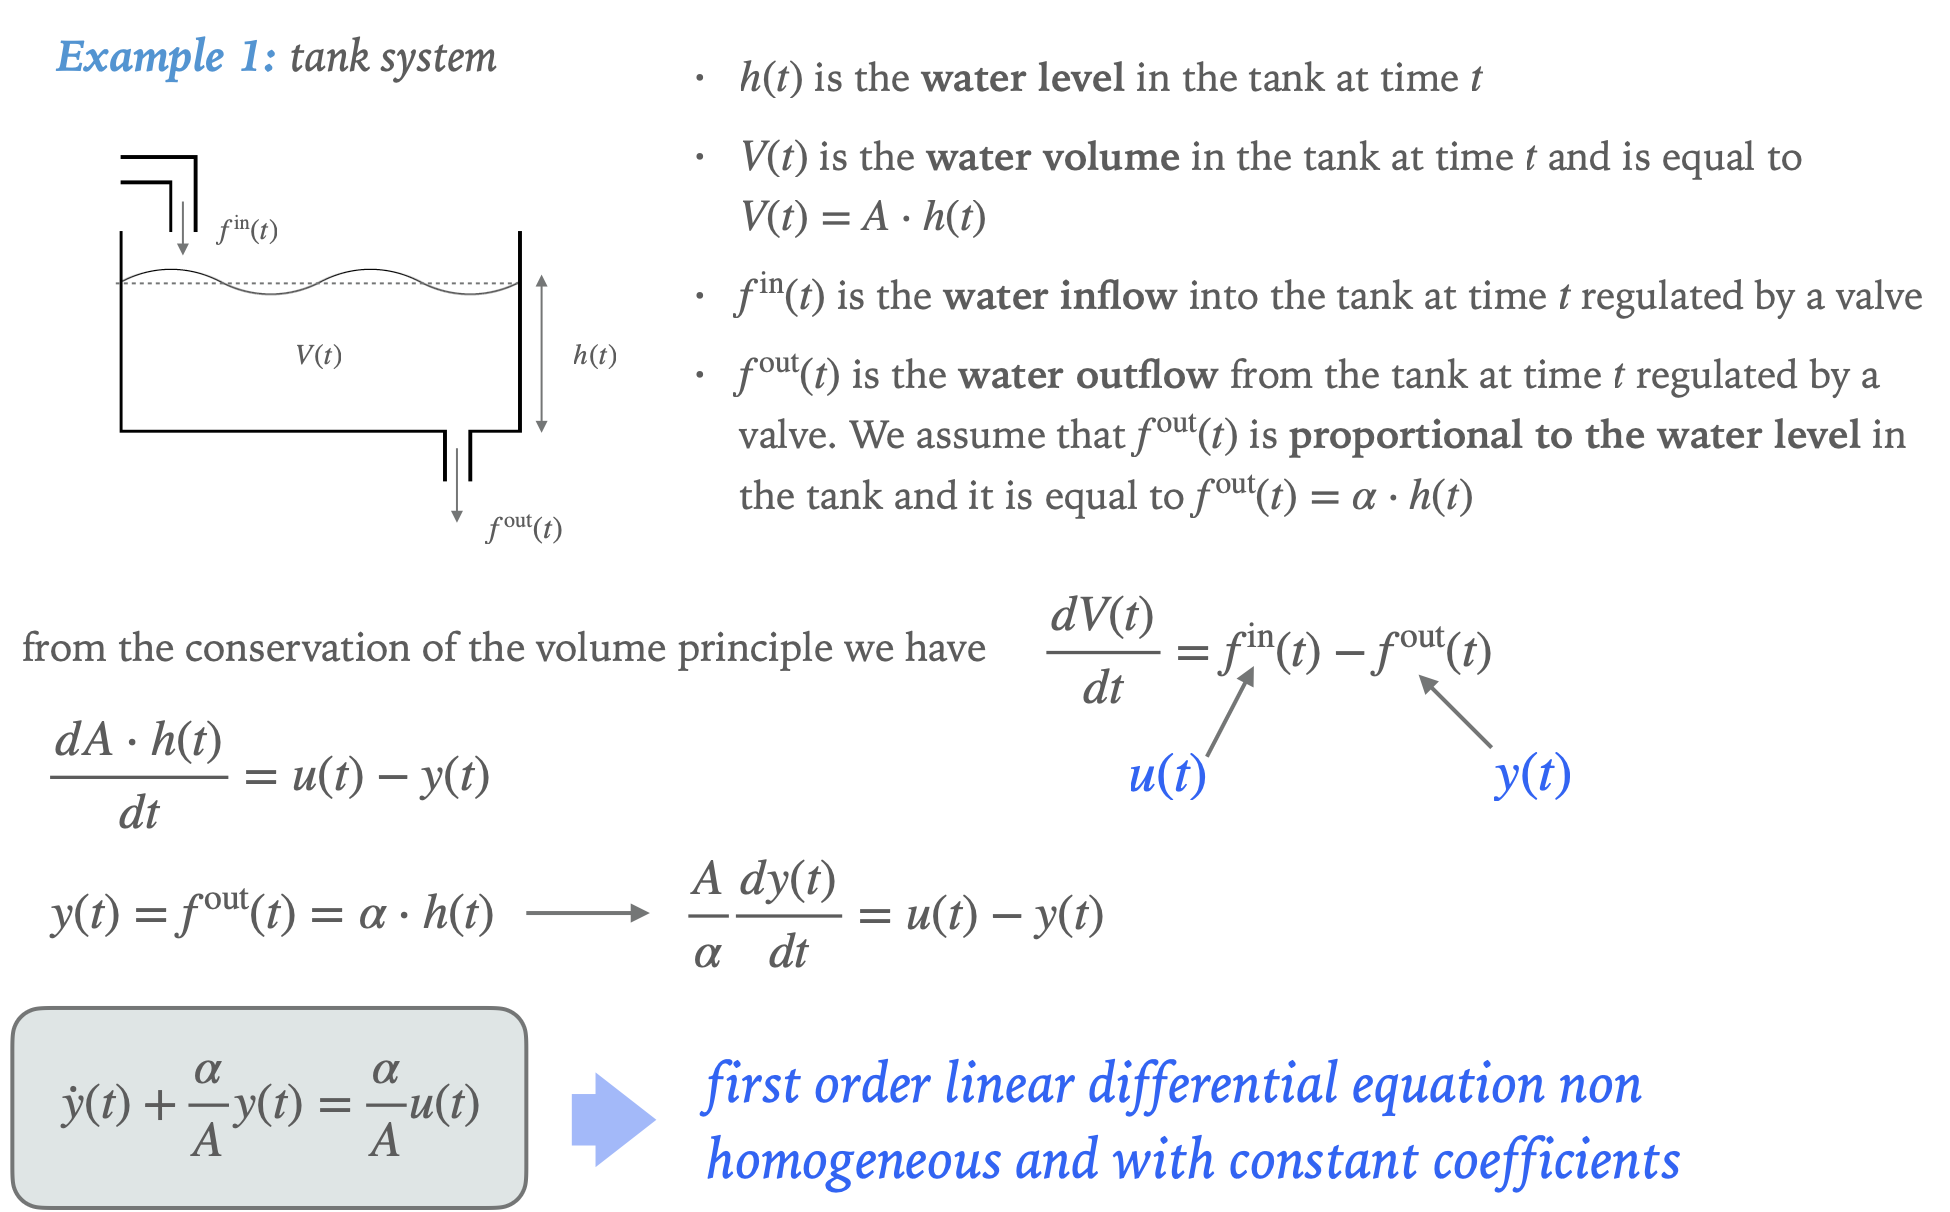
\includegraphics[width=1\textwidth]{../../images/tank_system.png}}
  \caption{A water tank system}
  \label{fig:tank_system}
\end{figure}

In continuous-time LTI systems, the relationship between input and output can always be described by a differential equation of order $n$ with constant coefficients that we need to solve only for $y(t)$.

\subsubsection{Input-Output LTI}
The general equation for an input-output Linear Time-Invariant system is
\begin{equation}
  y^n(t) + a_{n-1}y^(n-1)(t) + \dots + \dots a_1 y^\prime (t) + a_0 y(t) = b_m u^m (t) + b_{m-1} y^(m-1) (t) + \dots + b_1 u^\prime (t) + b_0 u(t)
\end{equation}

or a summed form
\begin{equation}
  \sum_{i=0}^n a_i \frac{d^i y(t)}{d t^i } = \sum_{i=0}^{m} b_i \frac{d^i u(t)}{d  t^i} 
\end{equation}

subject to 
\begin{itemize}
  \item $u,y : T \rightarrow \mathbb{R}$
  \item $n \geq m$
  \item $a_0, \dots, a_n \in \mathbb{R}$ and $a_n=1$
  \item $b_0, \dots, b_m \in \mathbb{R}$
\end{itemize}

In order to solve the linear differential equation and get the response of the system $y(t)$, we need to know the initial conditions of the output at $t=0$ and the applied input over time.
The total response of the system is given by two terms that can be separated output
\begin{equation}
  y(t) = y_n(t) + y_f(t)
\end{equation}

where $y_n(t)$ is the free response of the output that is obtained by having input equal to zero but with a non-zero initial condition and $y_f(t)$ is the forced response of the output which has an initial condition of the output equal to zero.
The free response $y_n(t)$ corresponds to finding the homogenous solution of the differential equation whereas $y_f (t)$ corresponds to finding the particular solution of the differential equations.

\subsubsection{State-Space Representation}
A system can also have more complexity than input-output relationships and may have a collection of parameters and information that are fully indicative of the system called the state.
Below is a digram of the previous vehicle example with the position added to the state as well as the input and output of acceleration and speed.
\begin{figure}[h]
  \centering
    \begin{tikzpicture}[baseline=(V.center)]
    \node[draw, rectangle, minimum width=2cm, minimum height=3cm] (V) {Vehicle};
    \draw[->] ($(V.west)+(-2,0.5)$) -- node[above] {Wheel} ($(V.west)+(0,0.5)$);
    \draw[->] ($(V.west)+(-2,0)$) -- node[above] {Pedal} ($(V.west)+(0,0)$);
    \draw[->] ($(V.west)+(-2,-0.5)$) -- node[above] {Brake} ($(V.west)+(0,-0.5)$);
    \draw[->] (V.east) -- node[above] {Speed} ($(V.east)+(3,0)$);
    \draw[->] (V.south) -- ++(0,-2) node[midway,right] {Position, Speed, Acceleration};
    \end{tikzpicture}
  \caption{Vehicle system with multiple inputs, one output, and state variables.}
  \label{figure:vehicle_system_with_state}
\end{figure}

Now, a causal system can be broken out into two equations
\begin{equation}
\begin{cases}
  \dot(\textbf{x})(t) = \phi(t_0, t, \textbf{x}(t), \textbf{u}(t)) & \text{Transition Function} \\
  \textbf{y}(t) = \eta(t, \textbf{x}(t), \textbf{u}(t)) & \text{Output Transform Function}
\end{cases}
\end{equation}

\begin{figure}[htbp]
  \centerline{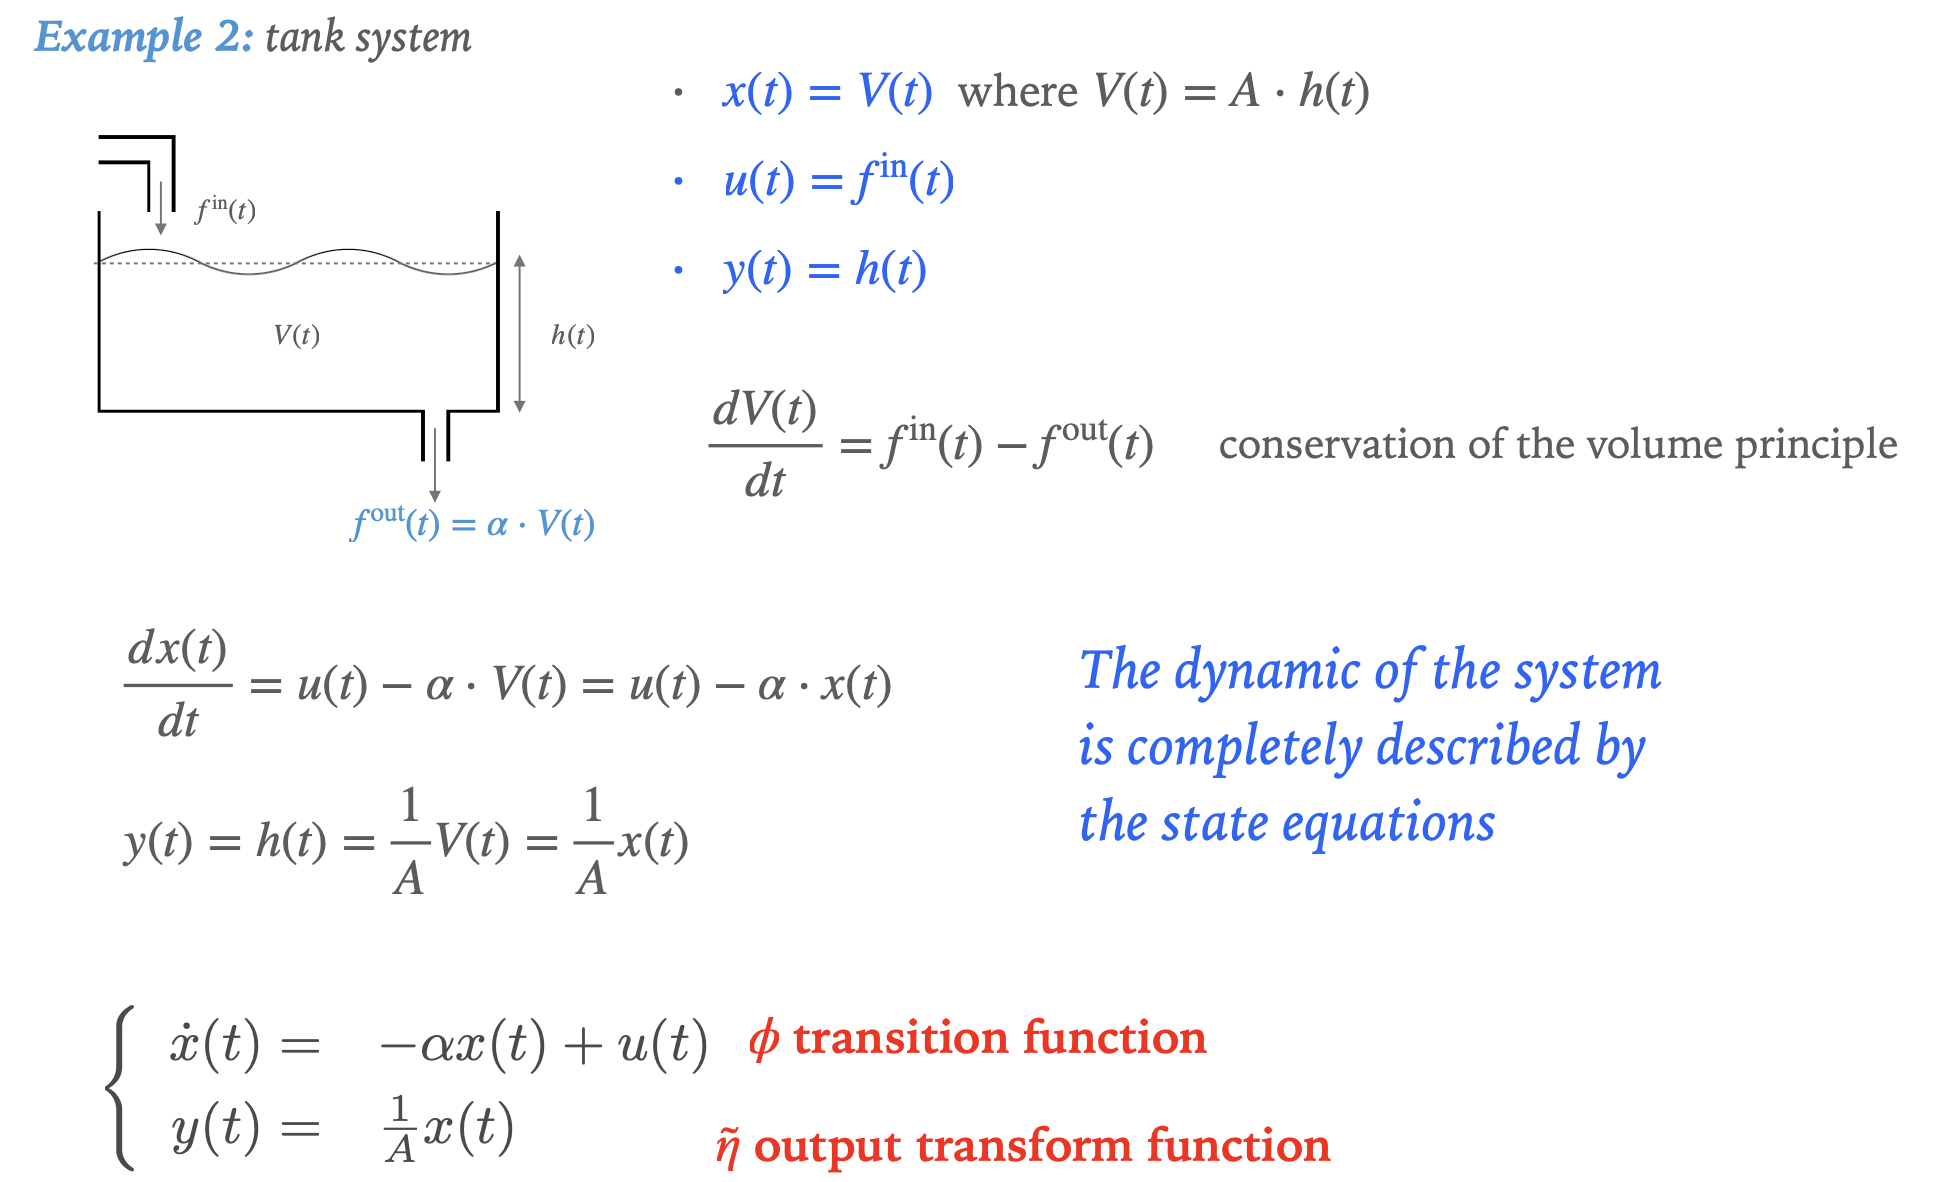
\includegraphics[width=1\textwidth]{../../images/tank_system_state.png}}
  \caption{The water tank example with state}
  \label{fig:tank_system_state}
\end{figure}

In this scenario, the transition function is a differential equation and the output transform function is an algebraic relationship.

\subsubsection{Matrix form State-Space}

We can write the state-space in matrix form for a SISO system
\begin{equation}
  \begin{cases}
    \dot{\textbf{x}}(t) = A \textbf{x}(t) + B u(t) \\
    y(t) = C^T \textbf{x} (t) + D u(t)
  \end{cases}
\end{equation}
where $A \in \mathbb{R}^{n \times n}, B, C \in \mathbb{R}^n, D \in \mathbb{R}$

For example, the following transition and output functions
\begin{equation}
  \begin{cases}
    \dot{x}_1 (t) = x_2 (t) \\
    \dot{x}_2 (t) = -\frac{k}{m} x_1 (t) - \frac{h}{m} x_2 (t) + \frac{1}{m} u(t) \\
    y(t) = x_1 (t)
  \end{cases}
\end{equation}

can be turned into the following set of matrix equations


\begin{align}
  \dot{\textbf{x}} (t) = 
  \begin{bmatrix}
      0 & 1 \\ - \frac{k}{m} & - \frac{h}{m}
  \end{bmatrix}
  \textbf{x} (t)
  +
  \begin{bmatrix}
    0 \\ \frac{1}{m}
  \end{bmatrix}
  u(t)
  , \quad
  y(t) =
  \begin{bmatrix}
    1 \\ 0
  \end{bmatrix}^\top 
  \textbf{x}(t)
\end{align}

\subsubsection{State Total Response}
Similar to the output response, we can break up the system state into the two forced and free terms.



\end{document}
